% !TEX root = ../main.tex
\chapter{Related Work} \label{ch:reated_work}

In this chapter, we give an overview of graph based algorithms
for image segmentation.
In \cref{sec:rw_hc} we will discuss hierarchical clustering 
methods.
Watershed methods will be explained in \cref{sec:rw_watershed_methods}
In \cref{sec:energy_based_methods} we will discuss
several energy based methods, show prototypical energy functions and
will give a brief overview how these energy functions can
be optimized.




%\section{Multicut}\label{sec:rw_multicut}
%% !TEX root = ../../main.tex

\section{Multicut}\label{sec:rw_multicut}

Segmentation is an important problem in computer vision as a first step
towards understanding an image. Many algorithms start with an over-segmentation
into superpixels, which are then clustered into ``perceptually meaningful''
regions.
Usually, the number of these regions is not known beforehand.

Recently, the multicut formulation~\cite{chopra_1993_mp}
(sometimes called \emph{correlation clustering}, \cite{bansal_2004_ml})
has become increasingly popular for unsupervised
image segmentation \cite{andres_2011_iccv,yarkony_2012_eccv,alush_2013_simbad}.

In this section we will give a brief overview of methods using multicut objectives
and will briefly introduce the multicut formulation.
The multicut and related work will be discussed extensively in \cref{ch:cgc} where
we propose a new solver for the such problems.

\paragraph{Problem Formulation:}
Given an edge-weighted region adjacency graph,
the problem is to find the segmentation which
minimizes the cost of the cut edges.
Therefore multicuts can be viewed as \emph{thresholding} w.r.t. close contours, while
naive thresholding will lead to inconsistencies 
(see \cref{fig:naive_thresholding} ).

Let $G=(V,E, \w)$ be a weighted region adjacency graph of
nodes $V$, representing superpixels,
and edges $E$.
%
The function $\w : E \rightarrow \mathbb{R}$ assigns a weight to each edge.
A positive weight expresses the desire that two adjacent nodes should
be merged, whereas a negative weight indicates
that these nodes should be separated into two different regions.
The \emph{multicut problem} can be written as a node labeling problem
\cite{bagon_2011_arxiv}:
%
\begin{align}
\argmin_{\Labels}
    \left\{
    \sum_{ e=(i,j) \in E}
        \w(e)
        \cdot \delta( \Labels_i \neq \Labels_j )
    \right\},
    \label{eq:multicut_primal_a}
\end{align}
%
where $\delta(a) = 1$ if $a$ is true and $0$ else.





\begin{figure}
\centering
\subfloat[Oversegmentation]{ \label{fig:naive_thresholding_a}
    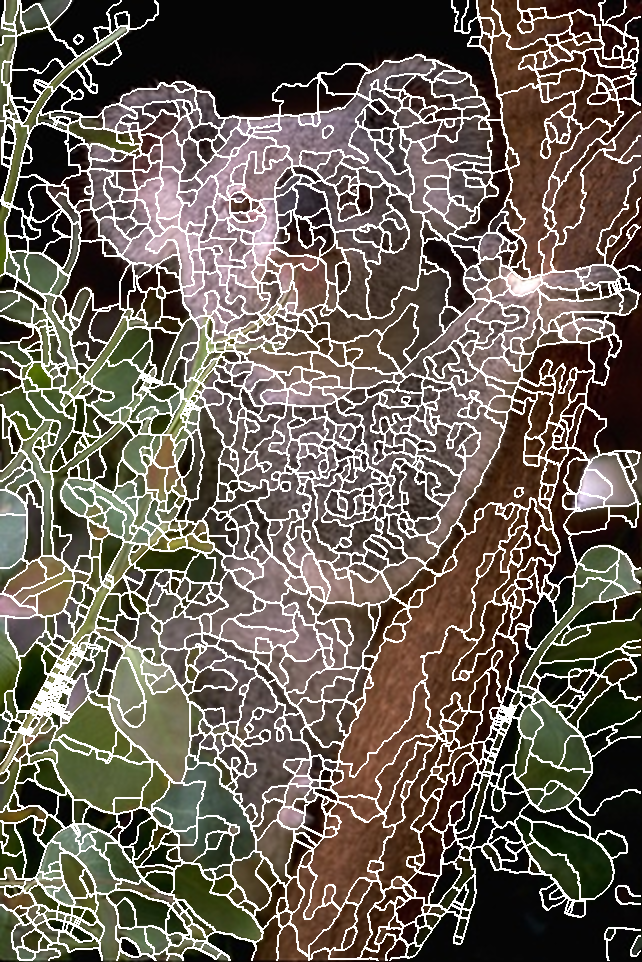
\includegraphics[width=0.25\textwidth]{fig/andres/0.png}
}
\subfloat[Oversegmentation]{  \label{fig:naive_thresholding_b}
    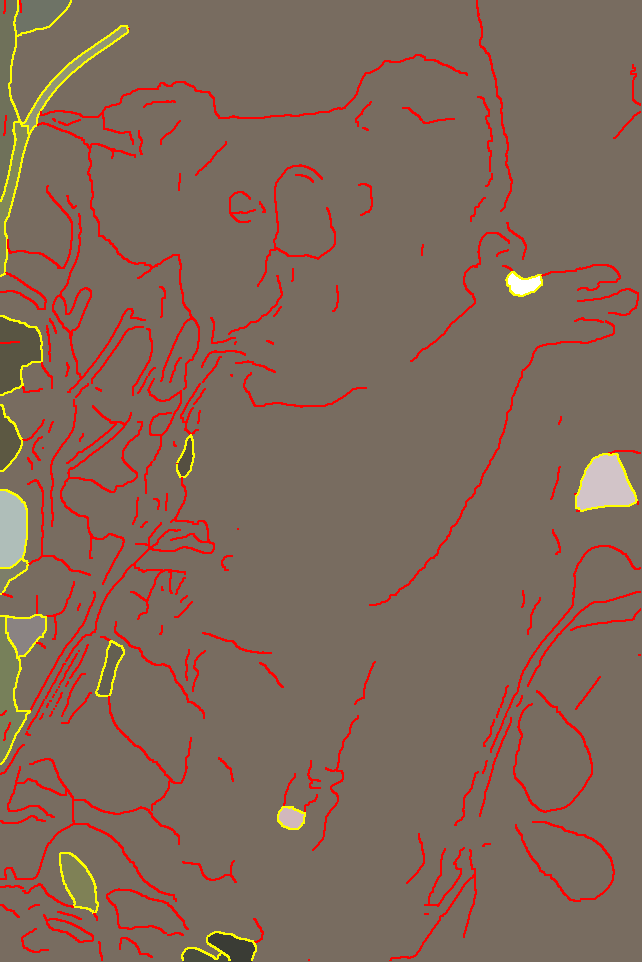
\includegraphics[width=0.25\textwidth]{fig/andres/1.png}
}
\subfloat[Oversegmentation]{  \label{fig:naive_thresholding_c}
    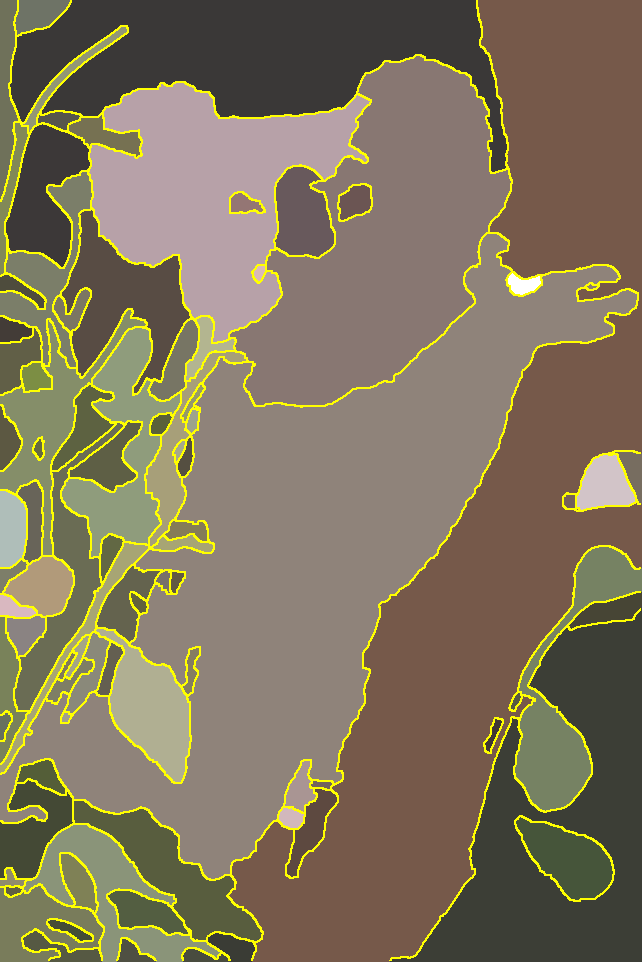
\includegraphics[width=0.25\textwidth]{fig/andres/2.png}
}
\addtocontents{lof}{%
    \vspace{1cm}
    \protect\centerline{%
        \protect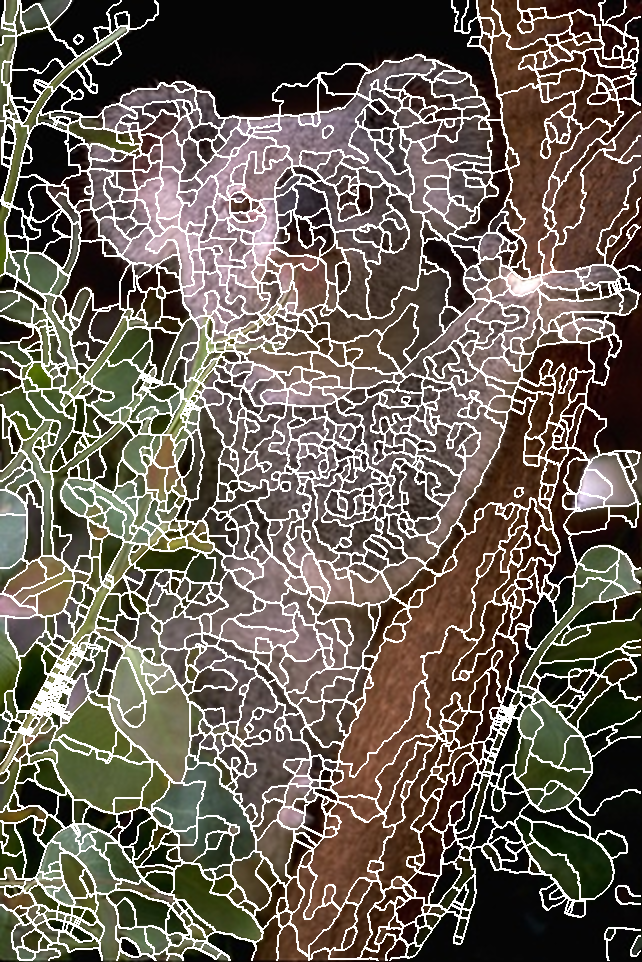
\includegraphics[width=.075\linewidth]{fig/andres/0.png}\hspace{0.2cm}
        \protect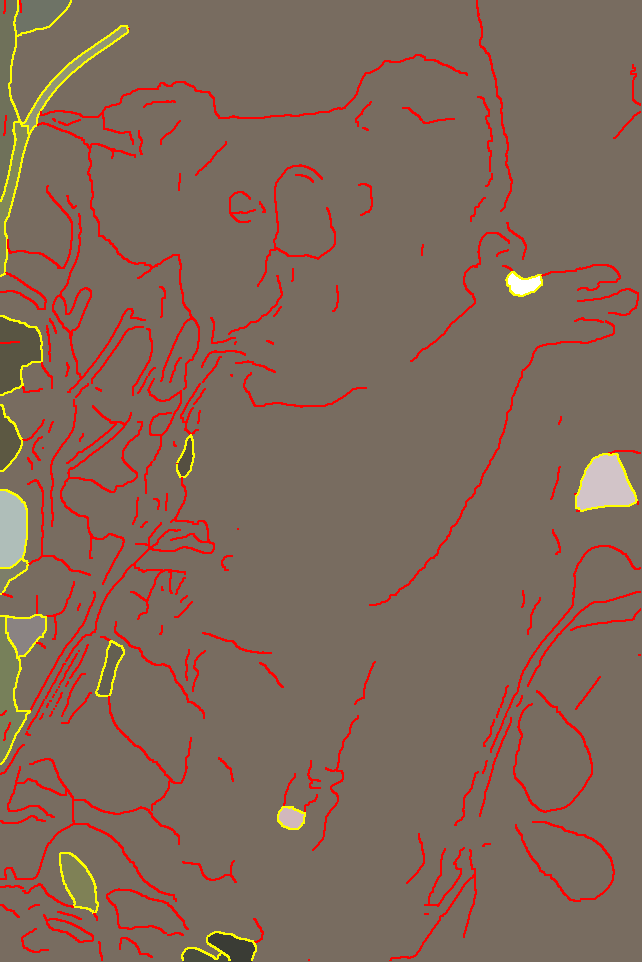
\includegraphics[width=.075\linewidth]{fig/andres/1.png}\hspace{0.2cm}
        \protect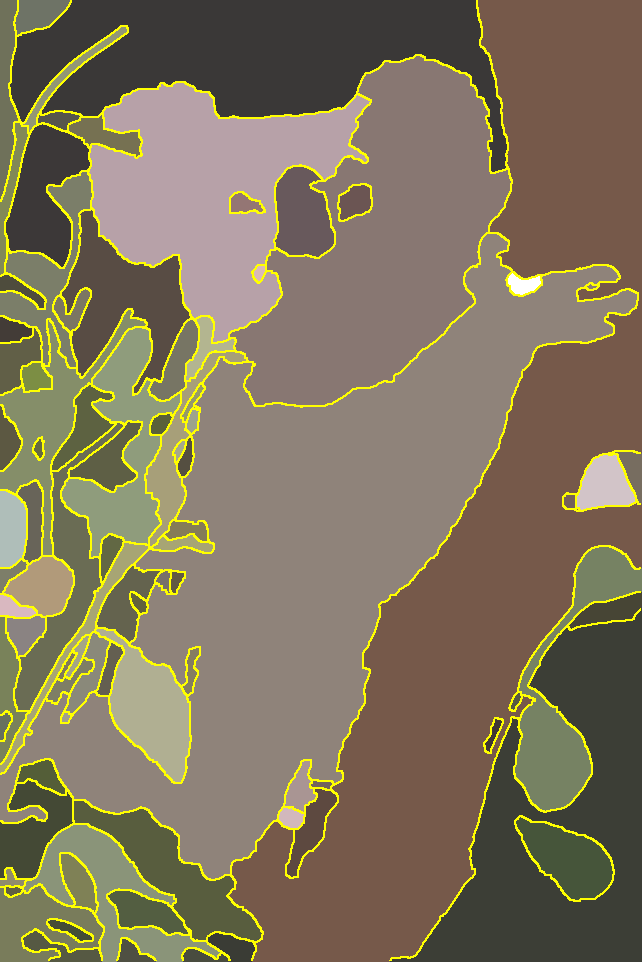
\includegraphics[width=.075\linewidth]{fig/andres/2.png} 
    }%
}%
\caption[Naive thresholding vs. multicuts]{
This figure has been taken from \cite{andres_2011_iccv} .
\Cref{fig:naive_thresholding_a} shows the oversegmentation of 
an image .
\Cref{fig:naive_thresholding_b} shows the result of naive thresholding..
Any inconsistent boundary is shown in red while consistent
boundaries are shown in yellow. 
\Cref{fig:naive_thresholding_c} shows the result with the multicut
constraints which lead to a meaningful segmentation.
} \label{fig:naive_thresholding}
\end{figure}


\citet{andres_2011_iccv} and \citet{kappes_2011_emmcvpr} use a
cutting plane approach where violated constraints are added
iteratively until no more violated constraints are found.


\begin{figure}
\centering
\subfloat[Superpixel Segmentation]{ \label{fig:mc_ineq_0}
    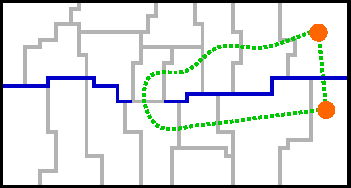
\includegraphics[width=0.4\textwidth]{fig/andres/ineq_0.pdf}
}
\subfloat[Corresponding Graph]{ \label{fig:ineq_1}
    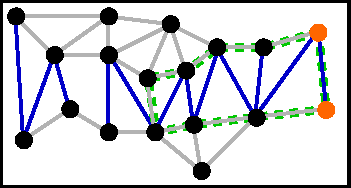
\includegraphics[width=0.4\textwidth]{fig/andres/ineq_1.pdf}
}
\addtocontents{lof}{%
    \vspace{1cm}
    \protect\centerline{%
        \protect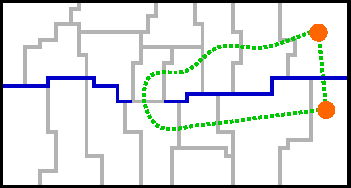
\includegraphics[width=.075\linewidth]{fig/andres/ineq_0.pdf}\hspace{0.2cm}
        \protect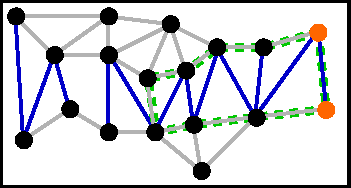
\includegraphics[width=.075\linewidth]{fig/andres/ineq_1.pdf}
    }%
}%
\caption[Violated multicut constraints]{
This figure has been taken from \cite{andres_2011_iccv} .
\Cref{fig:mc_ineq_0} shows the oversegmentation of 
an image .
\Cref{fig:mc_ineq_1} shows the corresponding graph.
} \label{fig:mc_ineq}
\end{figure}

 

%\section{Hierarchical Clustering}\label{sec:rw_hc}
% !TEX root = ../../main.tex
\section{Hierarchical Clustering}\label{sec:rw_hc}

%%%%%%%%%%%%%%%%%%%%%
%dendrogram
%%%%%%%%%%%%%%%%%%%%%%
\begin{figure}[H]
    \centering
    \subfloat[Bottom-Up: Nodes are merged with increasing time]{\label{fig:hc_bottom_up}
        {
            \begin{tikzpicture}[sloped]
                \node (a)    at (-6,0)      {a};
                \node (b)    at (-5,0)      {b};
                \node (c)    at (-4,0)    {c};
                \node (d)    at (-3,0)     {d};
                \node (e)    at (-2,0)       {e};

                \node (ab)   at (-5.5,1)    {};
                \node (cd)   at (-3.5,1)    {};
                \node (cde)  at (-2.75,2)       {};
                \node (all)  at (-4,3)    {};
                
                \node (root) at (-4,4) {root}; 

                \draw (a) |- (ab.center);
                \draw (b) |- (ab.center);
                \draw (c) |- (cd.center);
                \draw (d) |- (cd.center);
                \draw (e) |- (cde.center);
                \draw (cd.center) |- (cde.center);
                \draw (ab.center) |- (all.center);
                \draw (cde.center) |- (all.center);
                \draw (all.center) |- (root.center);

                \draw[->,-triangle 60] (-7,0) -- node[above]{time} (-7,4);
            \end{tikzpicture}
        }
    }\hspace{2cm}
    \subfloat[Top-Down: Nodes are divided with increasing time]{\label{fig:hc_top_down}
        {
            \begin{tikzpicture}[sloped]
                \node (a)    at (-6,0)      {a};
                \node (b)    at (-5,0)      {b};
                \node (c)    at (-4,0)    {c};
                \node (d)    at (-3,0)     {d};
                \node (e)    at (-2,0)       {e};

                \node (ab)   at (-5.5,1)    {};
                \node (de)   at (-2.5,1)    {};
                \node (cde)  at (-3.25,2)       {};
                \node (all)  at (-4,3)    {};
                
                \node (root) at (-4,4) {root}; 

                \draw (a) |- (ab.center);
                \draw (b) |- (ab.center);
                \draw (c) |- (cde.center);
                \draw (d) |- (de.center);
                \draw (e) |- (de.center);        
                \draw (de.center) |- (cde.center);
                \draw (ab.center) |- (all.center);
                \draw (cde.center) |- (all.center);
                \draw (all.center) |- (root.center);

                \draw [->,-triangle 60] (-7,4) -- node[below,align=center]{time} (-7,0);
            \end{tikzpicture}
        }
    }
    \addtocontents{lof}{%
    \vspace{1cm}
    \protect\centerline{%
    \protect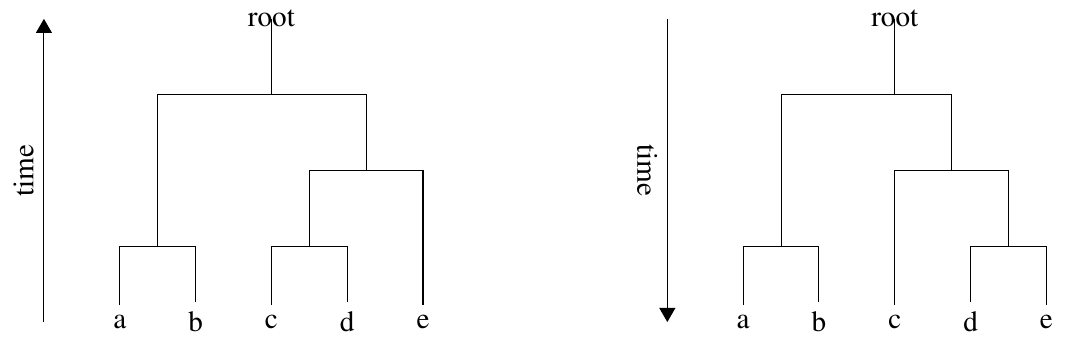
\includegraphics[width=.2\linewidth]{fig/thump/dendro.png}
    }%
    }%
    \caption[Bottom-up vs. top-down hierarchical clustering]{
        Bottom-Up clustering: Nodes are merged with increasing time.
        At the begin, all nodes are leafs, and they are merged
        together.
        Top-Down clustering: Nodes are divided with increasing time.
        At the begin, all nodes are in the root of the tree,
        and with increasing time, nodes are split.

    }
    \label{fig:hc_bottom_up_top_down}
\end{figure}


Hierarchical clustering techniques have been successfully used
in computer vision since decades \citep{ohlander_1978_cgip,forsyth_2002_book,arbelaez_2006_cvpr,iglesias_2013,morel_1995_book}.

The method  of \citet{ohlander_1978_cgip} is an example for \emph{top-down} clustering,
where all pixels start in one single cluster. Each cluster is recursively divided 
into  more clusters. The method proposed in \cref{ch:cgc} has a strong connection to
\emph{top-down} clustering.
\citet{arbelaez_2006_cvpr} and \citet{iglesias_2013} use the bottom-up approach,
also called \emph{agglomerative clustering}, where 
adjacent nodes in a graph are merged iteratively to create 
a set of nested segmentations.


Such a hierarchy of clusters can be visualized as a dendrogram (see \cref{fig:hc_bottom_up_top_down} ).
The dendrogram can be interpreted as a tree where each node represents a
region in the image.
The leafs in the tree are the atomic units of the image (e.g. pixels, super-pixels or super-voxels)
and the root note is the entire scene itself (e.g. the complete image / graph).

There are a few differences between classic unstructured agglomerative clustering
\citep{florek_1951,sokal_1958_science_bulletin,ward_63_jasa}
and agglomerative clustering on graph data structures \citep{arbelaez_2006_cvpr,iglesias_2013,morel_1995_book}, 
e.g. grid-graphs and region adjacency graphs\citep{vlachos_1993_csv}.
While in unstructured hierarchical clustering, any pair of observations can be merged,
for graph hierarchical clustering, only adjacent nodes / regions can be merged.
In the literature this is also called ``hierarchical clustering with connectivity constraints'' \cite{scikit_learn}.


The main idea behind agglomerative clustering is very simple:

Initially, all observations start in a single cluster. 
Next, clusters which have highest similarities will be merged
iteratively.
Due to this merging, similarities change and need to be updated
/ recomputed. Therefore  noisy initial features
 become more informative.


\begin{table}
\begin{scriptsize}
\begin{tabular}{ |l|l|p{5cm}|}
    \hline 
    Euclidean Distance
        & $||a-b||_2 = \sqrt{\sum{ (a_i-b_i })^2 } $
        & For low dimensional data \\  \hline 
    Squared Euclidean Distance
        & $||a-b||_2^2 = \sum{ (a_i-b_i })^2  $
        & For low dimensions data\\  \hline
    Manhattan Distance
        &  $||a-b||_1 = \sum{ |a_i-b_i |}  $
        & Multi purpose \\  \hline 
    $\mathcal{X}^2$-Distance  
        &  $\frac{1}{2}\sum{  \frac{(a_i-b_i)^2}{a_i+b_i} }$
        & For histograms \\  \hline 
    Earth Mover  Distance          
        &  see \citet{levina_2001_iccv} 
        & For histograms \\  \hline 

\end{tabular}

\end{scriptsize}
\caption{
    An overview of the most common distances measurements and their main properties.
}\label{tab:hc_distance_types}
\end{table}



\begin{table}
\begin{scriptsize}
\begin{tabular}{ |l|l|p{5cm}|}
    \hline
    Average Linkage \citep{sokal_1958_science_bulletin}           
        & $d_{al}(C_a,C_b) = \frac{1}{|C_a||C_b|} \sum _{a \in C_a} \sum_{b \in C_b} d(a,b) $ 
        & \scriptsize Prefers clusters with same variance \cite{sokal_1958_science_bulletin} \\ \hline

    Single Linkage \citep{florek_1951}            
        & $d_{sl}(C_a,C_b) =  \min\{d(a,b) : a \in C_a, b \in C_b\}$ 
        & Nice theoretic properties \citep{hartigan_1981_jjamstat,milligan_1980_psycho}, can lead
          to very irregular shaped clusters \\ \hline
    Complete Linkage \citep{sorensen_1948}         
        & $d_{cl}(C_a,C_b) =  \max\{d(a,b) : a \in C_a, b \in C_b\}$ 
        & Prefers clusters with same diameter \citep{milligan_1980_psycho} \\ \hline
    Centroid Distance         
        & $d_{cd}(C_a,C_b) =  d(\bar{C}_a,\bar{C}_b) $ 
        & Robust w.r.t. outliers \citep{milligan_1980_psycho} \\ \hline
    Wards Minimum Variance \citep{ward_63_jasa}
        & $d_{wmv}(C_a,C_b) = \frac{ d(\bar{C}_a,\bar{C}_b)}{ \frac{1}{|C_a|} + \frac{1}{|C_b|} } $ 
        & Prefers clusters with same size, is sensible to outliers \citep{milligan_1980_psycho} \\ \hline
\end{tabular}

\end{scriptsize}

\caption{
    The distance between to clusters is usually based on the 
    individual distance between elements within the clusters.
    These distance are \emph{linked} together.
    An overview of the most common cluster distances linkages and their main properties.
}\label{tab:hc_linkage_types}
\end{table}


The definition of a specific distance betweens clusters is crucial, 
but strongly depends on the application.
The distance between two clusters is usually based on the 
individual distance between elements within the clusters.
These distance are then \emph{linked} together using a specific linkage type.
\Cref{tab:hc_distance_types} gives a short overview of many common distance
types and \cref{tab:hc_linkage_types} gives a  brief overview 
of most common cluster linkage types and their main properties.








\iffalse
\begin{tikzpicture}[scale=  1,every node/.style={minimum size=1cm},on grid]
        
    %slanting: production of a set of n 'laminae' to be piled up. N=number of grids.
    

    %%%%%%%%%%%%%%%%%%%%%%%%%%%%%%%%%%%%%%%%%%%%%%%%%%%%%%%%%%%%%%%
    % 0 bottom layer
    %%%%%%%%%%%%%%%%%%%%%%%%%%%%%%%%%%%%%%%%%%%%%%%%%%%%%%%%%%%%%%%%
        
    \begin{scope}[yshift=0,every node/.append style={yslant=0.5,xslant=-1},yslant=0.5,xslant=-1]
        \draw[-latex,thick] (-0.17,3.21/2) node[right]{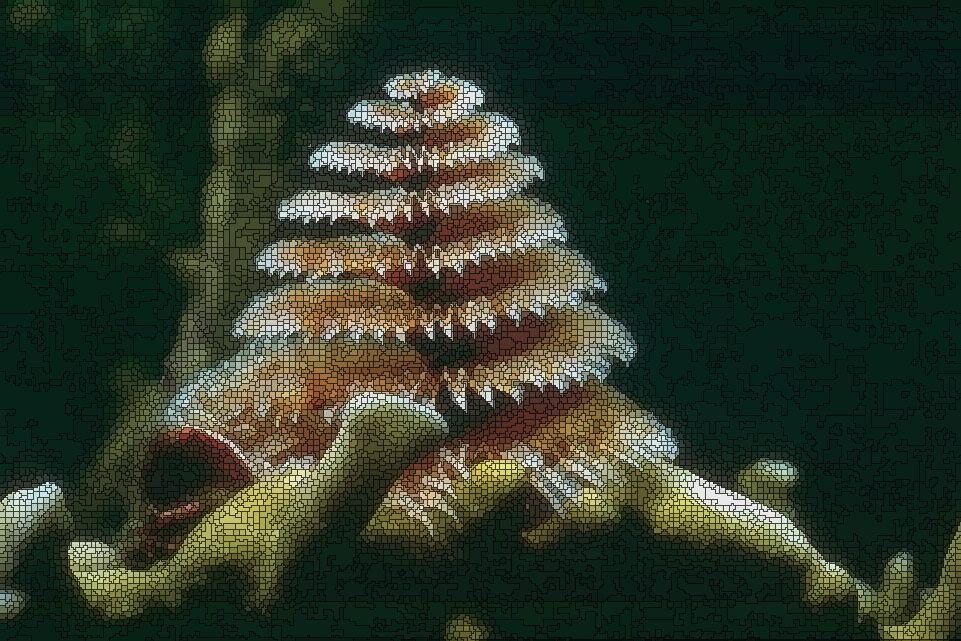
\includegraphics[width=4.82cm]{fig/12074/0.png}};
        \draw[black,very thick] (0,0) rectangle (4.81,3.21);
    \end{scope}

    \begin{scope}[yshift=60*1,every node/.append style={yslant=0.5,xslant=-1},yslant=0.5,xslant=-1]
        \draw[-latex,thick] (-0.17,3.21/2) node[right]{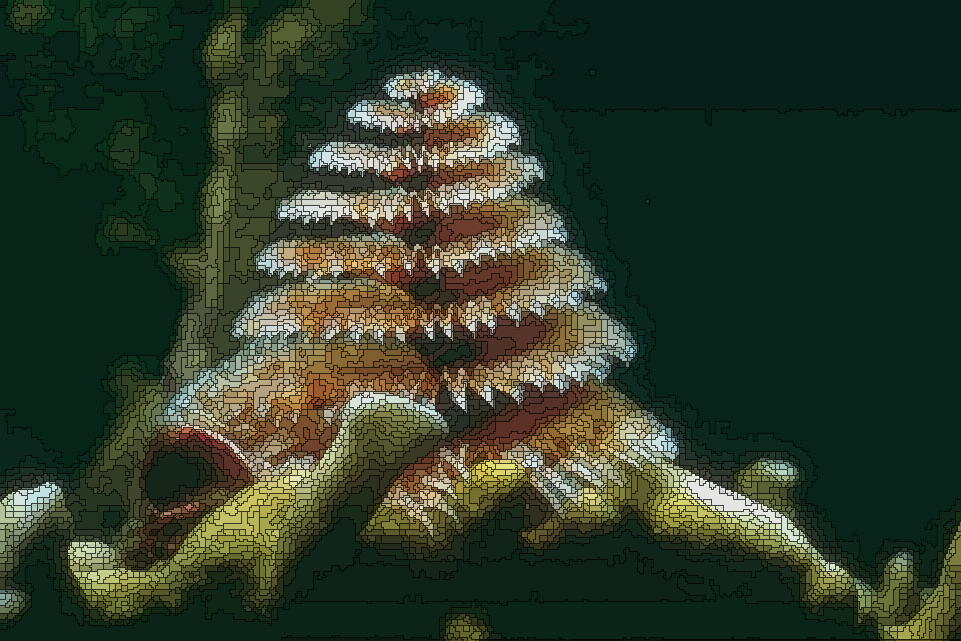
\includegraphics[width=4.82cm]{fig/12074/2.png}};
        \draw[black,very thick] (0,0) rectangle (4.81,3.21);
    \end{scope}

    \begin{scope}[yshift=60*2,every node/.append style={yslant=0.5,xslant=-1},yslant=0.5,xslant=-1]
        \draw[-latex,thick] (-0.17,3.21/2) node[right]{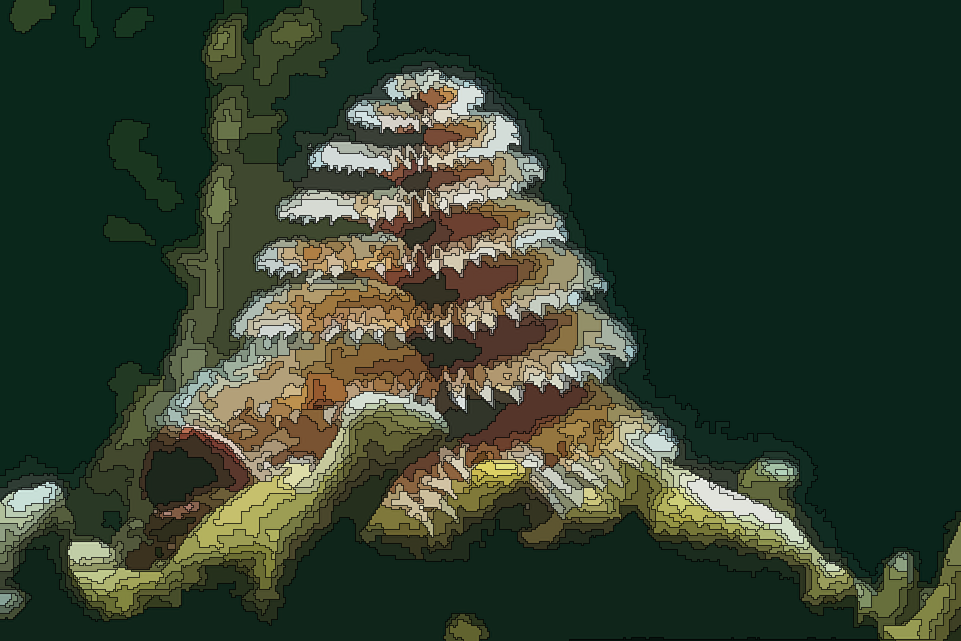
\includegraphics[width=4.82cm]{fig/12074/4.png}};
        \draw[black,very thick] (0,0) rectangle (4.81,3.21);
    \end{scope}

    \begin{scope}[yshift=60*3,every node/.append style={yslant=0.5,xslant=-1},yslant=0.5,xslant=-1]
        \draw[-latex,thick] (-0.17,3.21/2) node[right]{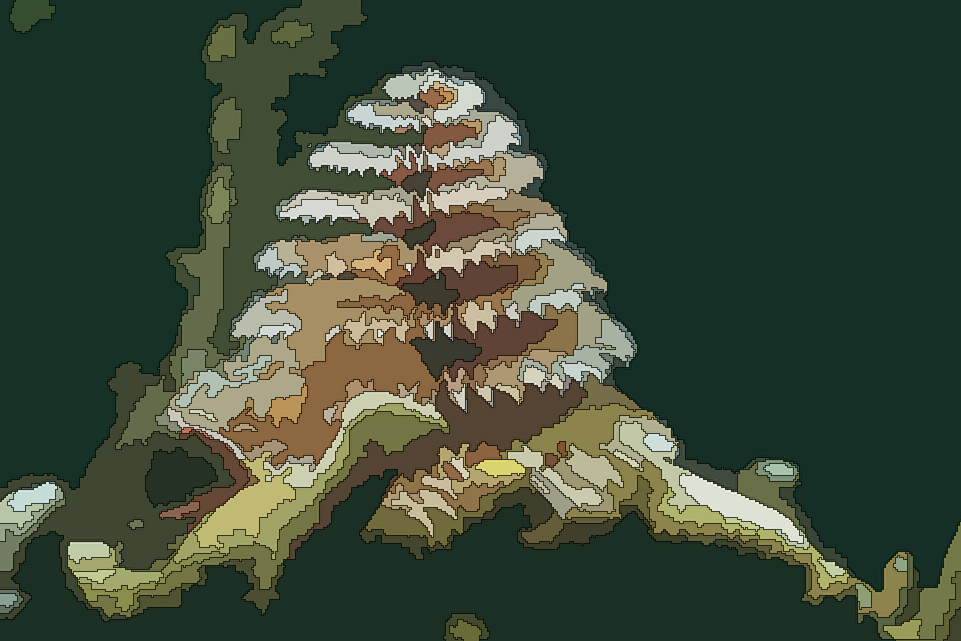
\includegraphics[width=4.82cm]{fig/12074/6.png}};
        \draw[black,very thick] (0,0) rectangle (4.81,3.21);
    \end{scope}

    \begin{scope}[yshift=60*4,every node/.append style={yslant=0.5,xslant=-1},yslant=0.5,xslant=-1]
        \draw[-latex,thick] (-0.17,3.21/2) node[right]{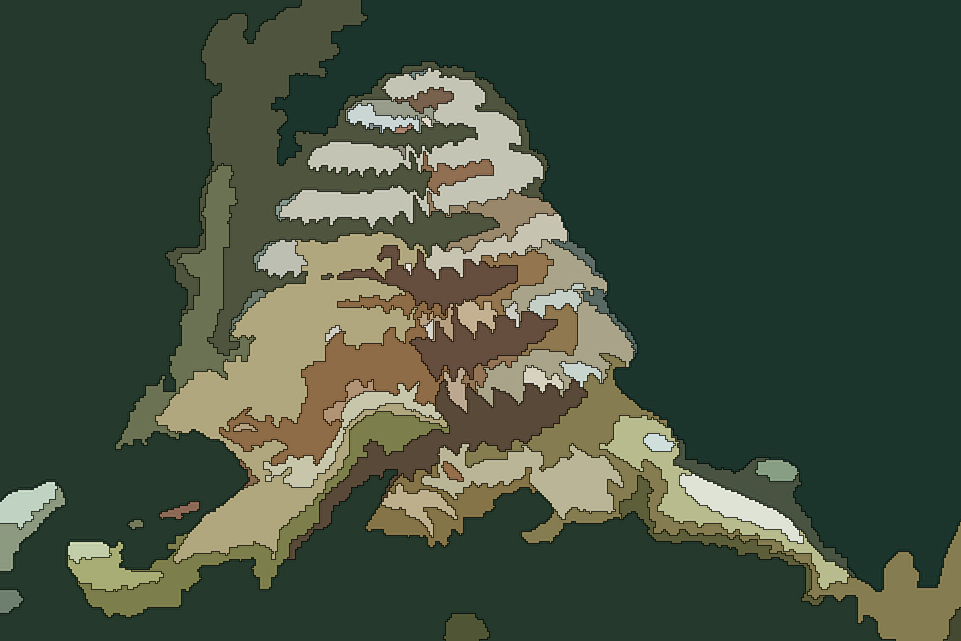
\includegraphics[width=4.82cm]{fig/12074/8.png}};
        \draw[black,very thick] (0,0) rectangle (4.81,3.21);
    \end{scope}


    \draw[->,-triangle 60] (-3,0) -- node[above]{time} (-3,4);

    %%%%%%%%%%%%%%%%%%%%%%%%%%%%%%%%%%%%%%%%%%%%%%%%%%%%%%%%%%%%%%%
    % 0 bottom layer
    %%%%%%%%%%%%%%%%%%%%%%%%%%%%%%%%%%%%%%%%%%%%%%%%%%%%%%%%%%%%%%%%
    \draw[-latex,thick] (6.2,2) node[right]{$\mathsf{over-segmentation}$}
         to[out=180,in=90] (4,2);
         
         
         
    %%%%%%%%%%%%%%%%%%%%%%%%%%%%%%%%%%%%%%%%%%%%%%%%%%%%%%%%%%%%%%%
    % 1 layer
    %%%%%%%%%%%%%%%%%%%%%%%%%%%%%%%%%%%%%%%%%%%%%%%%%%%%%%%%%%%%%%%%
    
    \draw[-latex,thick] (6.2,5.5) node[right]{$\mathsf{Region adjacency graph 1}$}
         to[out=180,in=90] (4,5.5);
\end{tikzpicture}
\fi







In the case of graph hierarchical clustering, informative features
can also be attached to the edges of the graph.
Edge detectors such as the gradient magnitude, gPb \citep{marie_2008_cvpr}  or learned
edge detectors \cite{dollar_2013_iccv}  can be used to boost performance
of agglomerative clustering \citep{arbelaez_2006_cvpr,iglesias_2013}.


\citet{ arbelaez_2006_cvpr} introduce the following notation:
They use $\Omega \in \mathbb{R}^2$ as image domain.
$P_0$ is the initial partition and they define a
\emph{hierarchical segmentation operator} (HSO) which
assigns a partition $P_\lambda$ given the initial partition and
a scale parameter $\lambda$.
Furthermore the following properties must be fulfilled for a HSO:  

\begin{align} 
P_{\lambda}  =  P_0 ,\hspace{0.5cm}  \forall \lambda \leq 0  \label{eq:ucm_hco_eq_0} \\ 
\exists \lambda_1 \in \mathbb{R}^+  : P_{\lambda}  =  \{ \Omega \} ,\hspace{0.5cm} \forall \lambda \geq \lambda_1  \label{eq:ucm_hco_eq_1} \\
\lambda < \lambda'  \rightarrow  P_{\lambda} \sqsubseteq   P_{\lambda'} \label{eq:ucm_hco_eq_2}
\end{align}


\Cref{eq:ucm_hco_eq_0} and \cref{eq:ucm_hco_eq_1}  give $\lambda$ a range.
\Cref{eq:ucm_hco_eq_2} ensures that the segmentations are nested.
They define the \emph{saliency} of a contour as the scale $\lambda$ where
the contour disappears (see \cref{fig:ucm_visu}).
Thresholding the saliency map leads to closed contours.
As a consequence, the complete hierarchical segmentation
generated by a HSO can be encoded in the saliency map (see \cref{fig:ucm_saliency}).


\citet{iglesias_2013} improve segmentation results by combining 
agglomerative clustering combined machine learning.
Their main idea is to combine training data at multiple scales
which are generated during the region merging process.
This approach outperforms single scale learning.


\begin{figure} 
    \begin{center}
        \subfloat[$K_0$]{ \label{fig:ucm_k0}
            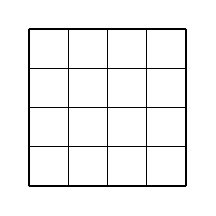
\begin{tikzpicture}
                \draw[step=0.5,black,thin] (0.0,0.0) grid (2,2);
                \draw[step=2,black,thick] (0.0,0.0) grid (2,2);
            \end{tikzpicture}
        }
        \hspace{0.5cm}
        %
        %
        %
        \subfloat[$K_1$]{ \label{fig:ucm_k1}
            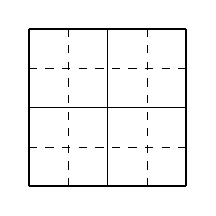
\begin{tikzpicture}
                \draw[step=0.5,black,very thin,dashed] (0.0,0.0) grid (2,2);
                \draw[step=1,black,thin] (0.0,0.0) grid (2,2);
                \draw[step=2,black,thick] (0.0,0.0) grid (2,2);
            \end{tikzpicture}
        }
        \hspace{0.5cm} 
        %
        %
        %
        \subfloat[$K_2$]{\label{fig:ucm_k2}
            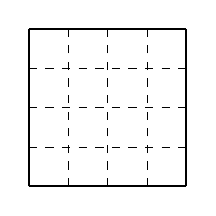
\begin{tikzpicture}
                \draw[step=0.5,black,very thin,dashed] (0.0,0.0) grid (2,2);
                \draw[step=2,black,thick] (0.0,0.0) grid (2,2);
            \end{tikzpicture}
        }
        \hspace{0.5cm}
        %
        %
        %
        \subfloat[$\mathcal{C}(\Upsilon) $]{ \label{fig:ucm_saliency}
            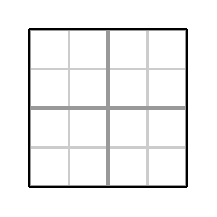
\begin{tikzpicture}
                \draw[step=0.5,black!20,thick] (0.0,0.0) grid (2,2);
                \draw[step=1,  black!40,very thick] (0.0,0.0) grid (2,2);
                 \draw[step=2,black,thick] (0.0,0.0) grid (2,2);
            \end{tikzpicture}
        }
        \hspace{0.5cm}
        %
        %
        %
        \subfloat[$\mathcal{C}(\Upsilon) $]{ \label{fig:ucm_saliency_3d}
            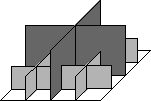
\includegraphics[width=0.2\textwidth]{fig/ucm3d.pdf}
        }
    \end{center}
    \addtocontents{lof}{%
    \vspace{1cm}
    \protect\centerline{%
        \protect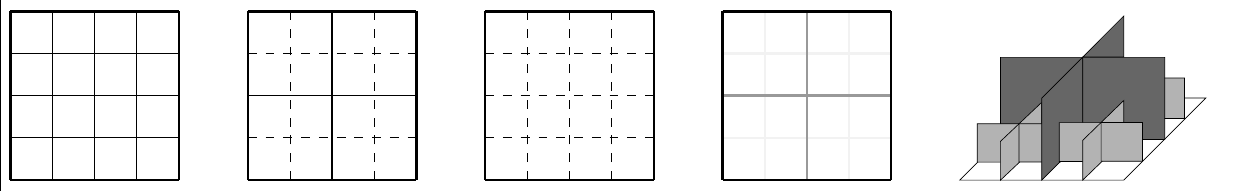
\includegraphics[width=.2\linewidth]{fig/thump/ucm.png} 
    }%
    }%
    \caption[Ultra metric contour map saliency]{
        \Cref{fig:ucm_k0} shows the a $4x4$ grid graph which serves as initial segmentation $K_0$.
        \Cref{fig:ucm_k1} shows the segmentation $K_1$ after the contraction of a few edges.
        Contracted edges are shown dashed.
        \Cref{fig:ucm_k2} shows the graph after all edges have been contracted.
        \Cref{fig:ucm_saliency} shows the saliency $\mathcal{C}$ of the contour $\Upsilon$.
        In \cref{fig:ucm_saliency_3d} the saliency from \ref{fig:ucm_saliency} is
        showed as a 3D visualization.
        This figure is very much inspired by \citep{arbelaez_2006_cvpr}.
    }\label{fig:ucm_visu}
\end{figure}




\Citet{najman_1994_sp} showed that there is a
strong connection between hierarchical segmentations
and watersheds.
They prove that there exists a bijection between
the set of ultrametric watersheds\citep{najman_2010_corr} and the set of hierarchical segmentations.
Furthermore, a recursive application of the watershed transformation  can
be used to generate a hierarchy of nested segmentations.
This transformation is called \emph{waterfall transformation} \citep{beuchner_1994_waterfall} .
 

%\section{Watershed Methods}\label{sec:rw_watershed_methods}
% !TEX root = ../../main.tex
\section{Watershed Methods}\label{sec:rw_watershed_methods}

The idea of watersheds has been introduced by \citet{beucher_1979_workshop}.

Other watersheds \citep{vinent_1991_pami,najman_1994_sp,roerdink_2000_finf,bertrand_2005_jmiv,cousty_2009_pami}.


The watershed algorithm can be often described with the following analogy:

\paragraph{Water Flooding:} A grayscale  image can be interpreted as hight map (see \cref{fig:ws_2d_map}, \cref{fig:ws_2d_map3d}).
The water level is raised as shown in \cref{fig:ws_a} - \cref{fig:ws_f}.
A watershed is wherever the water of two adjacent valleys is meeting (see \cref{fig:ws_e},\cref{fig:ws_f} and \cref{fig:ws_2d_lines}).


% watersheds illustrated
\begin{figure}
    \centering
    \subfloat[1d Image Data]{ \label{fig:ws_a}
        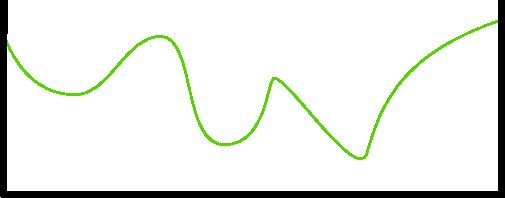
\includegraphics[width=0.25\textwidth]{fig/ws_no_no.pdf}
    }
    \hspace{0.5cm}
    \subfloat[Local minima]{  \label{fig:ws_b}
        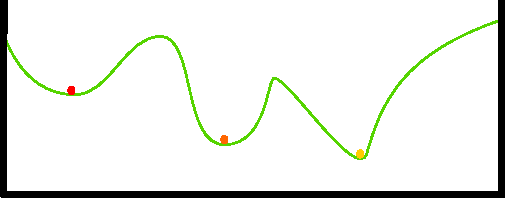
\includegraphics[width=0.25\textwidth]{fig/ws_no.pdf}
    }
    \hspace{0.5cm}
    \subfloat[flooding starts]{  \label{fig:ws_c}
        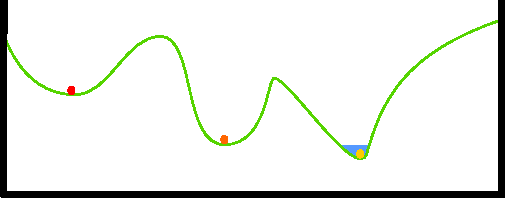
\includegraphics[width=0.25\textwidth]{fig/ws3.pdf}
    }
    \\
    \subfloat[flooding]{  \label{fig:ws_d}
        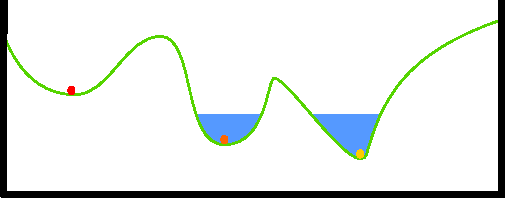
\includegraphics[width=0.25\textwidth]{fig/ws2.pdf}
    }
    \hspace{0.5cm}
    \subfloat[watershed 1]{  \label{fig:ws_e}
        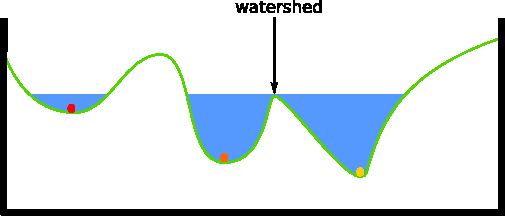
\includegraphics[width=0.25\textwidth]{fig/ws1.pdf}
    }
    \hspace{0.5cm}
    \subfloat[watershed 2]{ \label{fig:ws_f}
        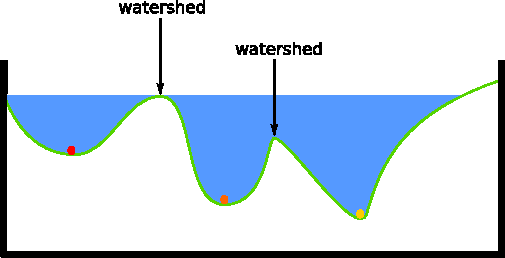
\includegraphics[width=0.25\textwidth]{fig/ws0.pdf}
    }
    \\ % 2D Watersheds
    \subfloat[$ $]{ \label{fig:ws_2d_map}
        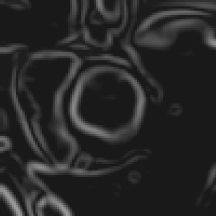
\includegraphics[height=0.26\textwidth]{fig/ws2d0.png}
    }
    \hspace{0.1cm}
    \subfloat[$ $]{ \label{fig:ws_2d_map3d}
        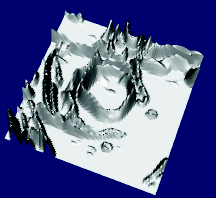
\includegraphics[height=0.26\textwidth]{fig/ws2d1.png} 
    }
    \hspace{0.1cm}
    \subfloat[$ $]{ \label{fig:ws_2d_lines}
        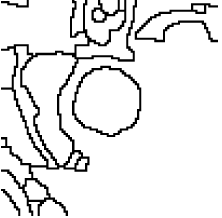
\includegraphics[height=0.26\textwidth]{fig/ws2d2.png}
    }

    \addtocontents{lof}{%
        \vspace{1cm}
        \protect\centerline{%
            \protect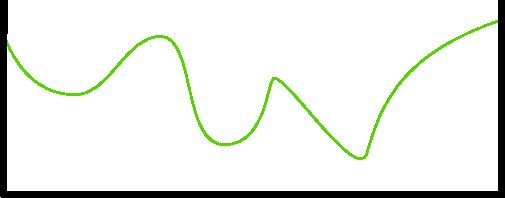
\includegraphics[width=.075\linewidth]{fig/ws_no_no.pdf}  \hspace{0.2cm}
            \protect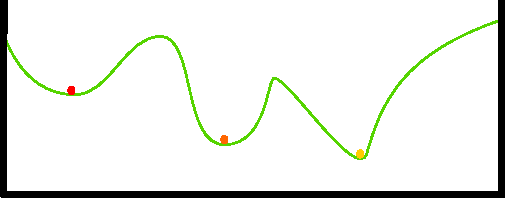
\includegraphics[width=.075\linewidth]{fig/ws_no.pdf}\hspace{0.2cm}
            \protect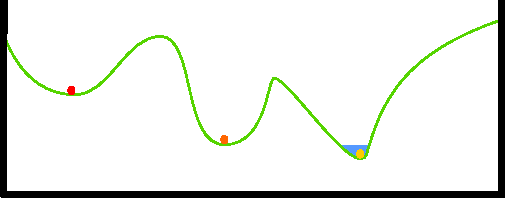
\includegraphics[width=.075\linewidth]{fig/ws3.pdf} 
        }%
        \vspace{0.2cm}
        \protect\centerline{%
            \protect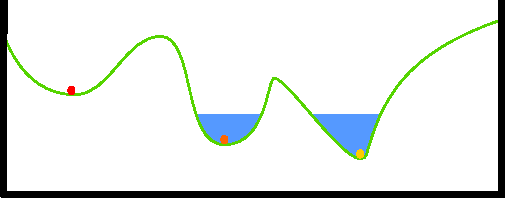
\includegraphics[width=.075\linewidth]{fig/ws2.pdf}  \hspace{0.2cm}
            \protect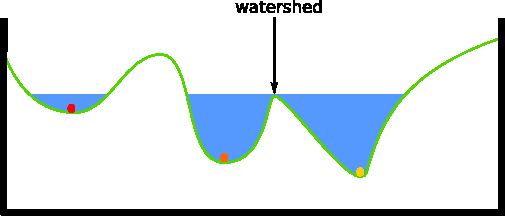
\includegraphics[width=.075\linewidth]{fig/ws1.pdf} \hspace{0.2cm}
            \protect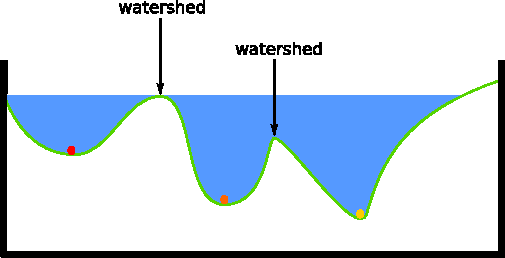
\includegraphics[width=.075\linewidth]{fig/ws0.pdf}%
        }%
        \vspace{0.2cm}
        \protect\centerline{%
            \protect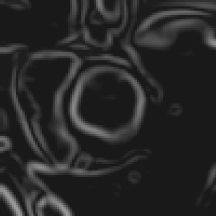
\includegraphics[height=.075\linewidth]{fig/ws2d0.png}  \hspace{0.2cm}
            \protect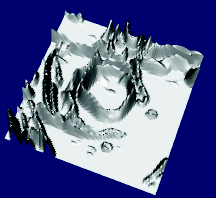
\includegraphics[height=.075\linewidth]{fig/ws2d1.png} \hspace{0.2cm}
            \protect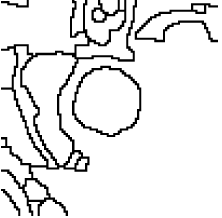
\includegraphics[height=.075\linewidth]{fig/ws2d2.png}%
        }%
    }%
    \caption[Illustration of watershed flooding process]{ 
        Illustration of watershed flooding process.
        The water level raises, and the watersheds are at the positions where water from different catchment basins is meeting.
    } \label{fig:watersheds_1d}
\end{figure}





\citet{couprie_2011_pami} proposed an algorithm, \emph{power-watershed}, a generalization of \citep{RANDOM_WALKER, boykov_2001_pami,vinent_1991_pami,najman_1994_sp,roerdink_2000_finf,bertrand_2005_jmiv,sinop_2007_iccv,cousty_2009_pami}.

They define the following model.
\begin{align}\label{eq:power_watershed}
\min_x \sum_{e_{ij} \in E}  w_{ip}^p |x_i-x_j|^q + \sum_{v_i } w_{Fi}^p |x_i|^q + \sum_{v_i } w_{Bi}^p |x_i-1|^q \\
s.t. \hspace{0.35cm} x(F)=1, \hspace{0.5cm} x(B)=0
\end{align}
Setting $p$ to 1 will lead to the methods proposed by \citet{sinop_2007_iccv}.
\Citet{allene_icv_2010} pointed out when $p=1$ and $q \rightarrow \infty$, solving
\cref{eq:power_watershed} is equivalent to applying a minimum spanning forest algorithm.




\citet{straehle_2011_miccai} proposed a watershed based method for interactive segmentation
of neural volume electron  microskopy images.
They show how a background prior be be efficiently integrated into watersheds,
and that this prior is beneficial for neuro data.
In addition \citet{straehle_2012_cvpr} proposed an uncertainty estimator for
guided interactive segmentation based on watersheds.
 

%\section{Energy Based Methods}\label{sec:energy_based_methods}
% !TEX root = ../../main.tex
\section{Energy Based Methods}\label{sec:energy_based_methods}

Energy based methods have recently become very popular.

Given a graph $G = (E,V)$ we 
associate  a variable $ x_i \quad \forall  u_i \in V$ with every node.
Within this thesis we focus on discrete energy functions,
therefore we use discrete variables $x$.
W.l.o.g. we set  $ x_i   \in \{ 0,1,2,\ldots, N_{labels}-1 \} \quad \forall \quad u_i \in V$,
which means that any node has the same number of labels.

An energy function $E(x)$ can be  defined  in the following way:

\begin{equation} \label{eq:gm_energy}
    E(x) = 
    \underbrace{
        \sum_{v \in V} \phi_i(x_i)
    }_{\text{unaries}}
     \quad +  \quad
    \underbrace{
        \sum_{e=(i,j) \in E } \phi_{ij}(x_i,x_j) 
    }_{\text{pairwise terms}}
\end{equation}



Here the \emph{unaries} $\phi_i(x_i)$ encode local costs
for a variable to have a certain label.
The \emph{pairwise terms} $\phi_{ij}(x_i,x_j) $ define the interaction of adjacent nodes.
Often they are used to introduce some smoothness prior
into the model \citep{szeliski_2008_pami}.
The vector which yields a minimum value of $E(x)$
is called $x_{\text{optimal}}$.
\begin{equation} \label{eq:gm_argmin}
x_{\text{optimal}} = \argmin_{x}  E(x)
\end{equation}

Before discussing how to optimize such energy functions,
we will give some concrete examples how $E(X)$ 
can be defined.



\paragraph{Denoising:}


Let $G=(V,E)$ be a grid graph corresponding to
a grayscale image.
Setting $N_{labels}$ to $256$ we can interpret  the variables $x$ directly as
gray values.
Let $I_i$ be the gray value of the pixel associated with variable $x_i$.

\begin{equation} \label{eq:gm_ef_dension}
E(x) = \sum_{v \in V}  (I_i - x_i)^2 + \sum_{e=(i,j) \in E } \lambda (x_i-x_j)^2
\end{equation}

The unaries ensure that the labeling matches the image.
The second order terms penalize adjacent nodes where the difference
between the labels is huge.
This model is described as part of a collection of MRF benchmark models \citep{szeliski_2008_pami}.




\begin{figure}[H]
    \centering
    \subfloat[Input Image $I$]{ \label{fig:eq:gm_ef_dension_input}
        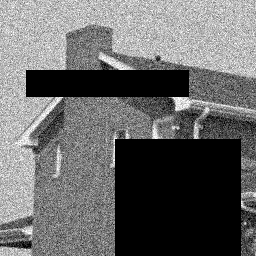
\includegraphics[width=0.25\textwidth]{fig/houseM-input.png}
    }
    \subfloat[ICM]{ \label{fig:eq:gm_ef_dension_icm}
        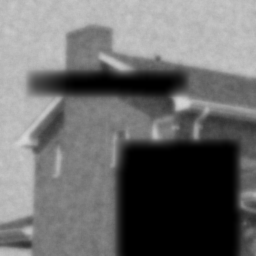
\includegraphics[width=0.25\textwidth]{fig/houseM-ICM.png}
    }
    \subfloat[$\alpha$-Expansion]{  \label{fig:eq:gm_ef_dension_ae}
        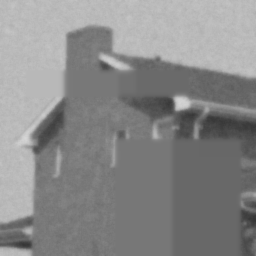
\includegraphics[width=0.25\textwidth]{fig/houseM-Expansion.png}
    }
    \subfloat[TRWS]{  \label{fig:eq:gm_ef_dension_trws}
        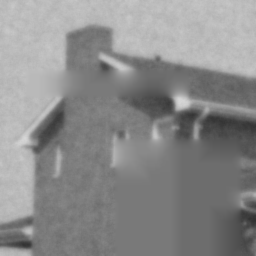
\includegraphics[width=0.25\textwidth]{fig/houseM-TRW-S.png}
    }
    \caption[Energy based truncated denoising]{
        Finding $x_{\text{optimal}} $ for the energy function given
        in \cref{eq:gm_ef_dension} is NP-hard. We show results of approximative solvers.
        Using \cref{fig:eq:gm_ef_dension_input} as input (for the black area no unaries 
        are used)
        the following
        results are obtained:
        ICM
         \citep{besag_1986_icm} (\Cref{fig:eq:gm_ef_dension_icm}) fails
        to fill the in-painting area. 
        While TRWS
        \citep{kolmogorov_2006_pami_trws}  (\Cref{fig:eq:gm_ef_dension_trws}) 
        and $\alpha$-Expansion
        \citep{boykov_2001_pami} (\Cref{fig:eq:gm_ef_dension_ae}) 
        can fill the in-painting area
        with meaningful values.
        The input image has been taken from \citep{szeliski_2008_pami}.
        The result images have been generated with OpenGM \citep{andres_2012_opengm_arxiv}.
    }\label{fig:gm_ef_denoise}
\end{figure}




\paragraph{Truncated Denoising:} 

This model is almost the same as the \emph{Denoising} model defined above,
but the second order term is clipped to $\gamma$ if $(x_i-x_j)^2$ is larger than $\gamma$.
Therefore one only pays $\gamma$ at strong edges.
Due to this truncation, the model allows for sharp edges.
This model is also described in \citep{szeliski_2008_pami}.


\begin{equation} \label{eq:gm_ef_dension_truncated}
E(x) = \sum_{v \in V}  (I_i - x_i)^2 + \sum_{e=(i,j) \in E } \lambda \cdot \min\left( (x_i-x_j)^2, \gamma\right)
\end{equation}

\begin{figure}[H]
    \centering
    \subfloat[Input Image $I$]{ \label{fig:eq:gm_ef_dension_truncated_input}
        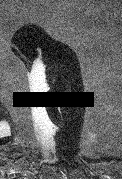
\includegraphics[width=0.25\textwidth]{fig/penguin-bar.png}
    }
    \subfloat[ICM]{ \label{fig:eq:gm_ef_dension_truncated_icm}
        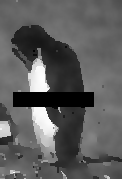
\includegraphics[width=0.25\textwidth]{fig/penguin-ICM.png}
    }
    \subfloat[$\alpha$-Expansion]{  \label{fig:eq:gm_ef_dension_truncated_ae}
        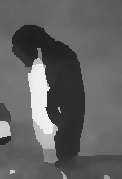
\includegraphics[width=0.25\textwidth]{fig/penguin-Expansion.png}
    }
    \subfloat[Trws]{  \label{fig:eq:gm_ef_dension_truncated_trws}
        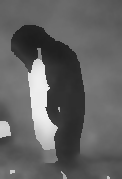
\includegraphics[width=0.25\textwidth]{fig/penguin-TRW-S.png}
    }
    \caption[Energy based truncated denoising]{
        Finding $x_{\text{optimal}} $ for the energy function given
        in \cref{eq:gm_ef_dension_truncated} is NP-hard. We show result of approximative solvers.
        Using \cref{fig:eq:gm_ef_dension_truncated_input} as input (for the black area no unaries 
        are used)
        the following
        results are obtained: ICM \citep{besag_1986_icm}  (\Cref{fig:eq:gm_ef_dension_truncated_icm}) fails
        to fill the in-painting area. While TRWS \cite{kolmogorov_2006_pami_trws}  (\Cref{fig:eq:gm_ef_dension_truncated_trws} ) 
        and $\alpha$-expansion \cite{boykov_2001_pami} (\Cref{fig:eq:gm_ef_dension_truncated_ae}) can fill the in-painting area
        with meaningful values.
        The input image has been taken from \citep{szeliski_2008_pami}.
        The result images have been generated with OpenGM\citep{andres_2012_opengm_arxiv}.
        In contrast to the result of \cref{eq:gm_ef_dension}, this model
        allows sharp edges.
    }\label{fig:gm_ef_dension_truncated}
\end{figure}


\paragraph{Ferromagnetic Ising model}
The ferromagnetic ising model consists 
of binary variables.
The unaries encode local costs for a variable
to take label $0$ or $1$.
The pairwise term is a smoothness prior, which penalizes
adjacent variables with different states.

\begin{equation} \label{eq:gm_ising}
    E(x) = 
    \underbrace{
        \sum_{v \in V} \phi_i(x_i)
    }_{\text{unaries}}
     \quad +  \quad
    \underbrace{
        \beta \cdot \sum_{e=(i,j) \in E }  \delta(\cdot x_i\neq x_j) 
    }_{\text{pairwise potts terms}} ,
\end{equation}
where $\delta(a)=1$ if $a$ is true and $0$ else
and $\beta>0$.

This model is also known as the \emph{potts model} and is often
used for binary segmentation (\eg\quad foreground background segmentation)
but can also be extended to the multi-label case.
Instead of a single $\beta$, often a different $\beta_i$ is used
for each edge \citep{szeliski_2008_pami}.



\begin{figure}[H]
    \centering
    \subfloat[Input Image $I$]{ \label{fig:eq:gm_ef_ising_input}
        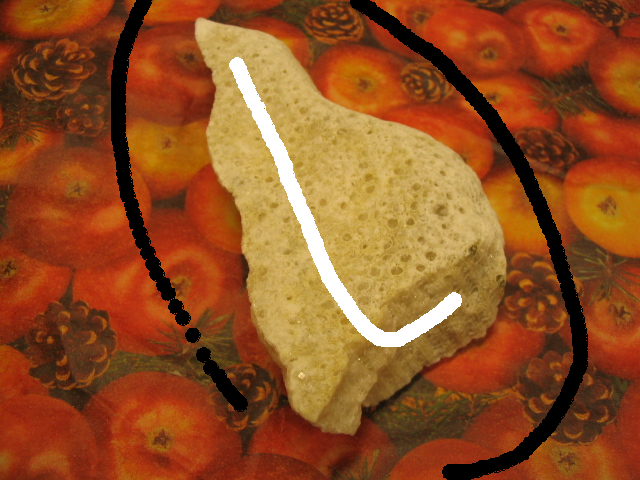
\includegraphics[width=0.25\textwidth]{fig/sponge.png}
    }
    \subfloat[ICM]{ \label{fig:eq:gm_ef_ising_icm}
        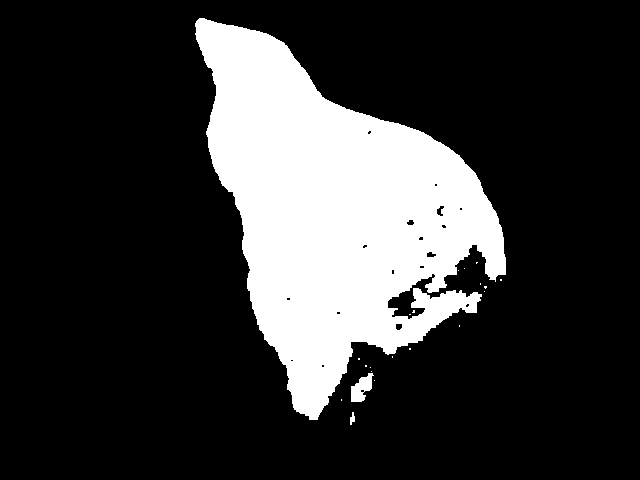
\includegraphics[width=0.25\textwidth]{fig/s_icm.png}
    }
    \subfloat[BP]{  \label{fig:eq:gm_ef_ising_bp}
        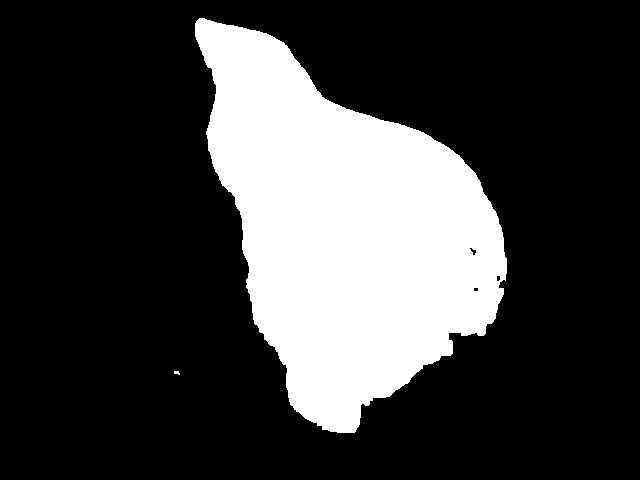
\includegraphics[width=0.25\textwidth]{fig/s_bp.png}
    }
    \subfloat[Graph Cut]{  \label{fig:eq:gm_ef_ising_cg}
        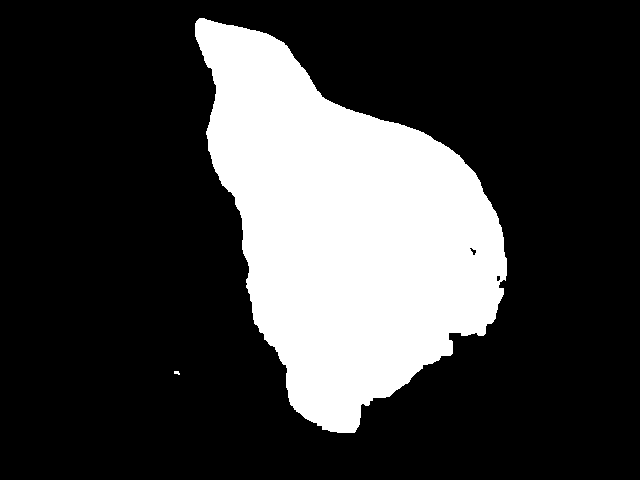
\includegraphics[width=0.25\textwidth]{fig/s_gc.png}
    }
    \caption[Potts Model]{ \label{fig:gm_ef_ising}
        Optimization results for the potts / ising model.
        A grid graph 4-neighborhood is used as input graph and 
        \cref{fig:eq:gm_ef_ising_input} shows the corresponding image.
        The unaries are based on a Gaussian mixture color models of foreground and background seeds defined by the user.
        The potts regularizer is modulated with the local constract.
        Since the model is submodular, graph cut finds optimal solutions (see \cref{sec:gcbased}).
    }
\end{figure}





\paragraph{Multicut Energy Function:}


Segmentation is an important problem in computer vision as a first step
towards understanding an image. Many algorithms start with an over-segmentation
into superpixels, which are then clustered into ``perceptually meaningful''
regions.
Usually, the number of these regions is not known beforehand.

Recently, the multicut formulation~\cite{chopra_1993_mp} 
(sometimes called \emph{correlation clustering}, \cite{bansal_2004_ml}) 
has become increasingly popular for unsupervised
image segmentation \cite{andres_2011_iccv,yarkony_2012_eccv,alush_2013_simbad}.


Given an edge-weighted region adjacency graph,
the problem is to find the segmentation which
minimizes the cost of the cut edges.
Therefore multicuts can be viewed as \emph{thresholding} w.r.t. closed contours, while
naive thresholding will lead to inconsistencies 
(see \cref{fig:naive_thresholding,fig:mc_ineq}).


\begin{figure}[h]
    \centering
    \subfloat[Oversegmentation]{ \label{fig:naive_thresholding_a}
        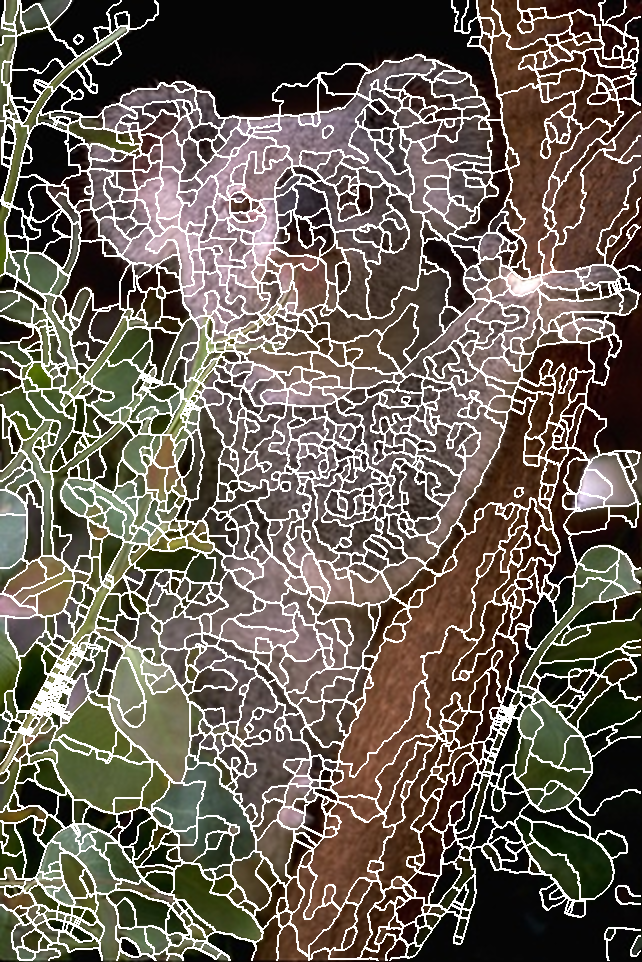
\includegraphics[width=0.25\textwidth]{fig/andres/0.png}
    }
    \subfloat[Inconsistencies]{  \label{fig:naive_thresholding_b}
        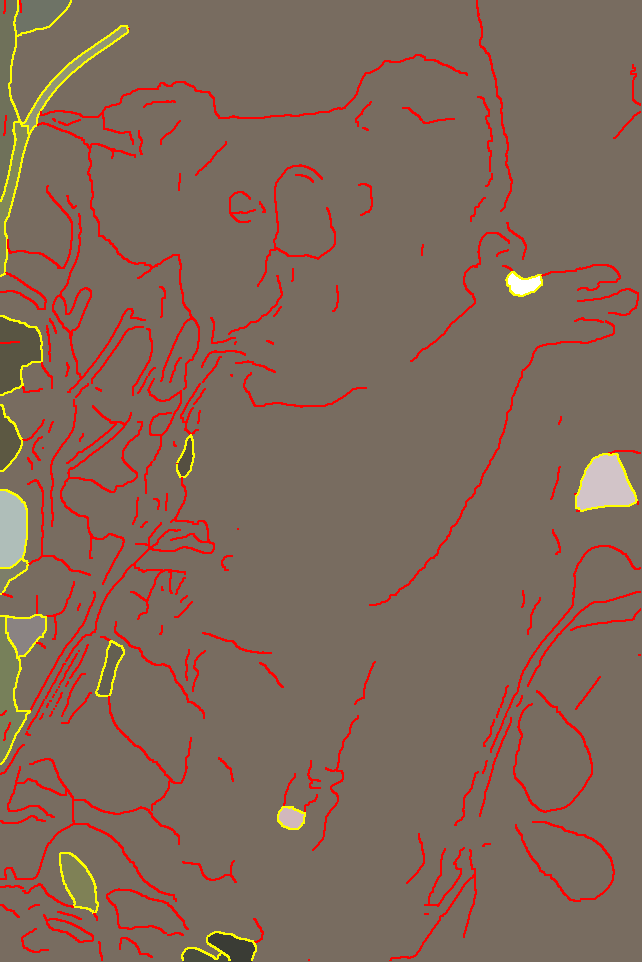
\includegraphics[width=0.25\textwidth]{fig/andres/1.png}
    }
    \subfloat[Consistent segmentation]{  \label{fig:naive_thresholding_c}
        \includegraphics[width=0.25\textwidth]{fig/andres/2.png}
    }
    \addtocontents{lof}{%
        \vspace{1cm}
        \protect\centerline{%
            \protect\includegraphics[width=.075\linewidth]{fig/andres/0.png}\hspace{0.2cm}
            \protect\includegraphics[width=.075\linewidth]{fig/andres/1.png}\hspace{0.2cm}
            \protect\includegraphics[width=.075\linewidth]{fig/andres/2.png} 
        }%
    }%
    \caption[Naive thresholding vs. multicuts]{
    This figure has been taken from \cite{andres_2011_iccv} .
    \Cref{fig:naive_thresholding_a} shows the oversegmentation of 
    an image.
    \Cref{fig:naive_thresholding_b} shows the result of naive thresholding.
    Any inconsistent boundary is shown in red while consistent
    boundaries are shown in yellow. 
    \Cref{fig:naive_thresholding_c} shows the result with the multicut
    constraints which lead to a meaningful segmentation.
    } \label{fig:naive_thresholding}
\end{figure}



Let $G=(V,E, \w)$ be a weighted region adjacency graph of
nodes $V$, representing superpixels,
and edges $E$.
%
The function $\w : E \rightarrow \mathbb{R}$ assigns a weight to each edge.
A positive weight expresses the desire that two adjacent nodes should
be merged, whereas a negative weight indicates
that these nodes should be separated into two different regions.


The \emph{multicut problem} can be written as a node labeling problem
\cite{bagon_2011_arxiv}:
%
\begin{align}
\argmin_{\Labels}
    \left\{
    \sum_{ e=(i,j) \in E}
        \w(e)
        \cdot \delta( \Labels_i \neq \Labels_j )
    \right\},
    \label{eq:multicut_primal_a}
\end{align}
%
where $\delta(a) = 1$ if $a$ is true and $0$ else.


Removing all unaries from \cref{eq:gm_energy} and 
setting $\phi_{ij}(x_i,x_j) =   \w_e \cdot \delta( x_i \neq x_j )$ 
will lead to the multicut objective (also see \cref{ch:cgc}) .

For planar problems  $N_{labels}$ can be set to 4 since any planar map is 4 colorable \citep{appel_1977_4color}.
For non-planar problems we need to set $N_{labels}$ to $|V|$.


\citet{andres_2011_iccv} and \citet{kappes_2011_emmcvpr} use a
cutting plane approach where violated constraints are added
iteratively until no more violated constraints are found (see fig \cref{fig:mc_ineq})

The multicut and related work will be discussed extensively in \cref{ch:cgc} where
we propose a new approximative solver for the such an objective.


\begin{figure}[h]
\centering
\subfloat[Superpixel Segmentation]{ \label{fig:mc_ineq_0}
    \includegraphics[width=0.4\textwidth]{fig/andres/ineq_0.pdf}
}
\subfloat[Corresponding Graph]{ \label{fig:mc_ineq_1}
    \includegraphics[width=0.4\textwidth]{fig/andres/ineq_1.pdf}
}
\caption[Violated multicut constraints]{
This figure has been taken from \cite{andres_2011_iccv}.
\Cref{fig:mc_ineq_0} shows the oversegmentation of 
an image .
\Cref{fig:mc_ineq_1} shows the corresponding graph.
Thresholding each edge individually will lead to violated constraints.
The current state of the edges  labeled as active (blue) or inactive (gray) is
inconsistent: Some nodes should be separated, since the edge between them is
active (blue), but there exists a path over inactive edges 
which connects these two nodes (showed in green).
\citet{andres_2011_iccv} and \citet{kappes_2011_emmcvpr} use a
cutting plane approach where these violated constraints are added
iteratively until no more violated constraints are found.
} \label{fig:mc_ineq}
\end{figure}




\subsection{Graph Cut Based Methods}\label{sec:gcbased}

If $N_{labels}=2$ and $\phi_{ij}(x_i,x_j)$ is submodular, 
graph cuts \cite{boykov_2001_pami,kolmogorov_2004_pami} can be applied to find $x_{\text{optimal}}$
in polynomial time.

Graph cut is an optimization algorithm which casts the energy minimizing problem
to an maximum flow / minimum cut problem. Energy functions of binary variables which
have the following form 

\begin{equation} \label{eq:gm_graph_cut_energy}
    E(x) = 
    \underbrace{
        \sum_{v \in V} \phi_i(x_i)
    }_{\text{unaries}}
     \quad +  \quad
    \underbrace{
        \sum_{e=(i,j) \in E } \phi_{ij}(x_i,x_j) 
    }_{\text{submodular pairwise terms}}
\end{equation}



and for which the pairwise energy term of binary variables is submodular, can be minimized with
graph cuts. 

$\phi_{ij}$ is submodular if:
\begin{equation} \label{eq:gm_submodular_criterion}
    \phi_{ij}(0,1) + \phi_{ij}(1,0) >  \phi_{ij}(0,0) + \phi_{ij}(1,1)
\end{equation}

To use graph cut, we have to associate each possible solution with a cut on a graph as in
\cref{fig:graph_cut} and ensure that the capacities on the graph match our energy function 
defined in \cref{eq:gm_graph_cut_energy}.
Since the max flow / min cut problem is defined on a directed graph, we have to construct
a directed graph from the energy function we want to minimize. We add a source and a
sink vertex and connect these terminal vertices with all variable vertices and assign
each edge a non-negative flow capacity. The flow goes from the source vertex to the
sink vertex. The edge capacities are constructed as described in the work of
\citet{kolmogorov_2004_pami}.

\Cref{fig:graph_cut_b} shows the
construction of  the directed max flow  graph, which is associated with the energy function $E(x)$.
\citet{kohli_2007_pami} proposed a method where graph cuts can be recomputed in an efficiently manner
if some capacities / energies where changed. This allows an efficient computation of 
graph cut min marginals an uncertainties \citep{kohli_2006_eccv,tarlow_2012_cvpr}.


\begin{figure}[H]
\begin{center}
\subfloat[$ $]{\label{fig:graph_cut_a}
    \includegraphics[height=0.3\textwidth]{fig/min_st.pdf}   
}
\hspace{1.5cm}
\subfloat[$ $]{\label{fig:graph_cut_b}
    \includegraphics[height=0.3\textwidth]{fig/min_st_d.pdf}   
}
\end{center}
\caption{
    \Cref{fig:graph_cut_a}: Each variable vertex is connected to the 2 terminal vertices, source s, and
        sink t, the edges between the variable vertices and terminal vertices are
        called t-links, the edges between variables vertices are called n-links. The
        line dotted in green is a cut, separating the variables with state zero from
        those with state one.
    \Cref{fig:graph_cut_b} is a simplification of the construction of the weighted graph.
        A constant term $\beta$ which has to be added to some capacities
        has been omitted for simplicity. 
        Interested readers are referred to  the work of \citet{kolmogorov_2004_pami}.
}\label{fig:graph_cut}
\end{figure}


Whenever we have an energy function of binary variables with pairwise potentials which
are non-submodular we cannot use graph cut. QPBO (quadratic pseudo-boolean optimization), 
the work of \citet{rother_2007_cvpr}, 
addresses the problem of minimizing such an energy function as the
following:

\begin{equation} \label{eq:gm_qpbo_energy}
    E(x) = 
    \underbrace{
        \sum_{v \in V} \phi_i(x_i)
    }_{\text{unaries}}
    \quad +  \quad
    \underbrace{
        \sum_{e=(i,j) \in E } \phi^{s}_{ij}(x_i,x_j)
    }_{\text{submodular pairwise terms}}
    \quad +  \quad
    \underbrace{
        \sum_{e=(i,j) \in E } \phi^{\bar{s}}_{ij}(x_i,x_j)
    }_{\text{non-submodular pairwise terms}}
\end{equation}

The basic idea of QPBO is to relax the problem by optimizing an auxiliary graphical
model with twice as many variables as the problem we want to optimize. The
auxiliary problem is constructed in such a way that it is submodular,
as showed in  \cite{rother_2007_cvpr}, and is optimized with graph cuts.
The output of QPBO
is a partial labeling $x_i \in \{ 0,1,\emptyset \}$, where $\emptyset$ is interpreted as unknown state. There are several
extension to QPBO which reduce the number
of variables which have an unknown state.

If the label space is larger than 2, $\alpha$-expansion and $\alpha \beta$-swap \cite{boykov_2001_pami} can be used.
The main idea of $\alpha$-expansion is to iteratively
solve binary sub-problems, where one only has to decide whether a variable should be
flipped to the state $\alpha$ or keep the current state. The value of $\alpha$ is changed in each iteration.

$\alpha \beta$-swap is very similar  to  $\alpha$-expansion.
But this time we have two labels, $\alpha$ and $\beta$. Within each iteration variables
with the state $\alpha$ can be flipped to the state $\beta$ and vice versa. The values of $\alpha$ and $\beta$
are changed after each iteration.

If the binary sub-problems are submodular graph cut can be used, otherwise QPBO.



\subsection{Linear Programming Methods}



An alternative formulation of the multicut objective (see \cref{eq:multicut_primal_a})
is in terms of binary edge indicator variables.
$\y \in \{0,1\}^{| E |}$:
\begin{align}
\argmin_{\y}
%
\left\{
    \sum_{e=(i,j) \in E} \w \left(e\right) \cdot \y_{e}
\right\}%
%
\;\;\text{s.t.}\;\;\y \in \MC_G.
\label{eq:multicut_dual_a}
\end{align}
%
%
$\text{MC}_G$ is the set of all multicut
constraints \cite{chopra_1993_mp} for graph $G$ forming
the so called \emph{multicut polytope}.
The objective in \cref{eq:multicut_dual_a}
is linear w.r.t. indicator variables $\y_{e}$.

In general,
$\y \in \MC_G$ can be enforced by an exponential number of
constraints \cite{chopra_1993_mp}, but in practice
-- for a given objective function --
a small subset of those are sufficient.
Therefore, a major branch of research has focused 
on cutting plane approaches,
by solving a relaxation of \eqref{eq:multicut_dual_a}
by a sequence of linear programs 
\cite{kim_2011_nips,kim_2012_ip,kappes_2013_arxiv,finley_2005_ml}.









Linear  programming methods methods can be used to optimize 
any discrete energy function, if the energy function is 
linearized.
To optimize an energy functions as the following,

\begin{equation} \label{eq:gm_nl_energy}
    E(x) = 
     \sum_{v \in V}
    \underbrace{
        \phi_i(x_i)
    }_{\text{unaries}}
     \quad +  \quad
     \sum_{e=(i,j) \in E } 
    \underbrace{
        \phi_{ij}(x_i,x_j) 
    }_{\text{pairwise terms}}
\end{equation}

we introduce $\mu_{i}^{l}$ as an indicator variable where $\mu_{i}^{l}=1$ indicates $x_i=l$.
In the same manner we use $\mu_{ij}^{l_a l_b}$ to indicate pairwise 
assignments.

The  constraints in \crefrange{eq:gm_lp_s}{eq:gm_lp_e} are
called \emph{local consistency constraints} \citep{sontag_2010_thesis}.

The constraints ensure that the indicator variables $\mu_{i}^{l}$ are consistent 
with pairwise indicators $\mu_{ij}^{l_a l_b}$ .
\begin{align}
    E(\mu) = \sum_{v \in V} \sum_{l=0}^{L_{\text{max}}} \label{eq:gm_lp}
    \mu_{i}^{l} \cdot \phi_{i}( l)
    \quad +  \quad
    %
    \sum_{e \in E} \sum_{l_a=0}^{L_{\text{max}}} \sum_{l_b=0}^{L_{\text{max}}}
    \mu_{ij}^{l_a l_b} \cdot \phi_{ij}( l_a,l_b) \\
    %
    s.t. \quad  \label{eq:gm_lp_s}
    \sum_{l=0}^{L_{\text{max}}} \mu_{i}^{l} = 1 \quad \forall \quad v_i \in V \\
    %
    \sum_{l_b=0}^{L_{\text{max}}} \mu_{ij}^{l_a l_b} = \mu_i 
    \quad \forall \quad e_{ij} \in E, 
    \quad l_a \in \{ 0,1,\ldots,L_{\text{max}} \} \\ 
    %
    \sum_{l_a=0}^{L_{\text{max}}} \mu_{ij}^{l_a l_b} = \mu_j 
    \quad \forall \quad e_{ij} \in E, 
    \quad l_b \in \{ 0,1,\ldots,L_{\text{max}} \} \\ 
    %
    \mu_i^l \geq 0 \quad \forall \quad v_{i} \in V,
    \quad l \in \{ 0,1,\ldots,L_{\text{max}} \}\\
    \mu_{ij}^{l_a l_b} \geq 0 \quad \forall \quad e_{ij} \in E,
    \quad l_a,l_b \in \{ 0,1,\ldots,L_{\text{max}} \} \label{eq:gm_lp_e}
\end{align}

Solving the LP in \cref{eq:gm_lp} will lead to fractional
solutions since the \emph{local consistency constraints} 
define a polytope which is a relaxation
of the marginal polytope.
In \cref{fig:local_poly} is a visualization of the local
polytope.
%  \footnote{
% Interested readers are refereed to the doctoral
% thesis of  \citet{sontag_2010_thesis} which gives
% a great overview and introduction to linear programming
% based optimization.
% }.

An additional set of constraints, \emph{integer constraint} as defined in \cref{eq:integral_constraint}, can be added to the LP in \cref{eq:gm_lp}. These constraints turn the LP into an integer LP (I-LP).

\begin{align}
    \mu_i^l \in \{0,1\} \quad \forall \quad v_{i} \in V,
    \quad l \in \{ 0,1,\ldots,L_{\text{max}} \} \label{eq:integral_constraint}
\end{align}

Solving the I-LP to optimality, will lead to 
global optimal solutions of the energy function defined in 
\cref{eq:gm_nl_energy}.







\begin{figure}[H]
\centering
\includegraphics[width=0.6\textwidth]{fig/frac_vert2.pdf}
\caption{
    A sketch of the local consistency polytope.
    The local polytope is a relaxation
    of the marginal polytope (red dashed lines).
    While the marginal polytope has only integral
    nodes (red nodes), the local polytope 
    will introduce fractional vertices which are shown
    in blue.
    The figure has been taken from \citep{sontag_2010_thesis}
    and has been modified slightly.
    Interested readers are referred to the doctoral
    thesis of  \citet{sontag_2010_thesis} which gives
    a great overview and introduction to linear programming
    based optimization.
}\label{fig:local_poly}
\end{figure}





 

%\section{MST Methods}\label{sec:rw_mst_methods}
%% !TEX root = ../../main.tex
\section{MST Methods}\label{sec:rw_mst_methods}
Discuss the method from \citet{felzenszwalb_2004_ijcv}.
Discuss the method from \citet{Straehle_k-smallestspanning}. 

%\section{Random Walker}\label{sec:rw_random_walker}
%% !TEX root = ../../main.tex
\section{Random Walker}\label{sec:rw_random_walker}

gready random waler 





%\section{Normalized Cuts}
